\documentclass{beamer}
%%%%%% UNOFFICIAL ICL BEAMER TEMPLATE V.0.1 %%%%%%
% This is a basic LaTeX Beamer template that I customised to have the logo of ICL and a background picture. Mind that this is NOT an official ICL template but it may still be useful for informal presentations.
% The official ICL graphical identity resources can be found here: http://www3.imperial.ac.uk/graphicidentity
% Please drop me an e-mail or comment via Twitter @AJunyentFerre if you found this was useful or have any suggestion to improve it.
%%%%%%

\usepackage[english]{babel}
\usepackage{tikz}
\usetikzlibrary{arrows.meta,positioning,fit,backgrounds}

%%%%%% THE FOLLOWING FILE CONTAINS THE STYLE DEFINITIONS %%%%%%
%%%%%% STYLE DEFINITIONS — inlined from the source deck's header.tex, so this
%%%%%% file is the whole deck (the build offers slides.tex as a download).
\usepackage[utf8]{inputenc}

\definecolor{gris}{rgb}{0.92,0.92,0.92}
\definecolor{blau-upc}{rgb}{.192,.365,.506}

\setbeamercolor{titlelike}{fg=blau-upc}
% \setbeamercolor{barra}{bg=white,fg=white}
\setbeamercolor{capcalera}{bg=blau-upc,fg=white}
\setbeamercolor{section in toc}{fg=blau-upc}
\setbeamertemplate{sections/subsections in toc}[circle]
\setbeamertemplate{itemize items}[circle]
\setbeamercolor{item}{fg=blau-upc}
\setbeamertemplate{blocks}[rounded][shadow=true]
\setbeamercolor*{block body}{bg=gris}
\setbeamerfont{block body}{size=\footnotesize}
\setbeamercolor*{block title}{parent=structure,bg=blau-upc,fg=white}

\setbeamersize{text margin left=12mm,text margin right=12mm}
\setbeamertemplate{navigation symbols}{}

\defbeamertemplate*{headline}{infolines theme}
{
	\begin{beamercolorbox}[wd=\paperwidth,ht=9.5mm,right]{white}%
		% (the ICL template's logo sat here; the empty box keeps the headline's height)
		\vskip0.2ex
	\end{beamercolorbox}
% 	\begin{beamercolorbox}[wd=\paperwidth,ht=0.5mm,left]{barra}%
% 		\hspace*{1mm}
% 	\end{beamercolorbox}
}

\setbeamertemplate{footline}
{
	\hbox{
	\begin{beamercolorbox}[wd=0.1\paperwidth,ht=10mm,left]{}
% 		\hspace*{1ex}\includegraphics[height=8mm]{./logotips/imperiallogo.pdf}\vskip 2ex
	\end{beamercolorbox}
	\begin{beamercolorbox}[wd=0.8\paperwidth,ht=3ex,center]{}
		\hspace*{4ex}\insertsection\vskip 4ex
	\end{beamercolorbox}
	\begin{beamercolorbox}[wd=0.1\paperwidth,ht=3ex,right]{}
		\insertpagenumber\hspace*{6ex}\vskip 4ex
	\end{beamercolorbox}
	}
}

\setbeamertemplate{title page}
{
	\vbox{}
	\vfill
	\begin{centering}
		{\usebeamerfont{title}\usebeamercolor[fg]{title}\inserttitle}
		\vskip0.2em
		{\usebeamerfont{subtitle}\usebeamercolor[fg]{subtitle}\insertsubtitle}
		\vskip2em\par
		\small\insertauthor\par
		\vskip0.7em\par
		\tiny\insertdate\vskip1em\par
	\end{centering}
% 	\vfill
}

% (the ICL template's background picture sat here)
%%%%%%
%%%%%%

%%%%%% TITLE, AUTHOR, DATE DEFINITIONS %%%%%%
\title{Agent Foundations}
\author{Daniel C}
\date{19th April 2026}
%%%%%%

\begin{document}


\frame{\titlepage}\section{Introduction}


\frame{\frametitle{Why Agent Foundations?}
	\begin{block}{Aligning a system that doesn't exist yet}
		{\tiny
		\begin{itemize}
			\item Alignment may eventually require us to steer a system far more capable than anything we have built, under conditions unlike anything we have yet observed
			\item Agent foundations studies the properties that capable agents tend to share \textit{in general}, rather than the details of any one system -- giving us a way to reason about highly capable agents \textit{in advance} of being able to study them directly
            \item At a sufficiently dangerous capability level, we may need to get key safety properties right on the \textit{first critical try}: a serious failure could be unrecoverable, leaving no room for the trial-and-error that science normally relies on
			\item Even if we learn about capable agents empirically from weaker systems, we still need a theory of \textit{which} properties continue to hold as capability increases -- and supplying that theory is itself the work of agent foundations
		\end{itemize}
		}
	\end{block}
}


\section{Reflective Stability}
\frame{\frametitle{Reflective Stability}
	\begin{block}{Self-modification and the stability of goals}
		{\tiny
		\begin{itemize}
			\item A sufficiently capable agent may be able to: rewrite its own source code, build a more capable successor, and radically revise its world model (e.g.\ learning new physics, ontology shifts)
			\item A property is \textit{reflectively stable} if it remains invariant under all such self-modifications
			\item A safety property we instil only matters if it is reflectively stable: a guardrail is of little use if the agent can self-modify to remove it, or build a successor that lacks it
			\item For a sufficiently capable goal-directed agent, the working assumption is that \textbf{a property persists only if there is some reason it has to} -- architectures, constraints, and conceptual schemes are all candidates for being optimised away under enough pressure
			\item So to guarantee a safety property holds (e.g.\ ``this system does not cause a catastrophe''), it is not enough to instil it once; we need it to be \textit{invariant under self-modification}, and we need to understand what kinds of properties \textit{can} have that invariance
		\end{itemize}
		}
	\end{block}
}


\frame{\frametitle{Two Pathways of Impact: Modelling vs.\ Implementation}
	\begin{block}{Modelling}
		{\tiny
		\begin{itemize}
			\item Build an \textit{abstract mathematical model} of an idealised, highly capable agent, and use it to make safety claims about how such an agent would behave
			\item The model need not be runnable; its value is that it lets us reason about such agents \textit{in advance}, and in particular show \textit{why} a given alignment proposal would fail
		\end{itemize}
		}
	\end{block}
    \begin{block}{Implementation}
		{\tiny
		\begin{itemize}
			\item Develop a theory to the point where it could be turned into an actual algorithm or running system that we could build and inspect
			\item On this pathway, researchers often favour \textit{modular} architectures -- a separate, inspectable world model, a planning module, and an explicit representation of the goal -- rather than one opaque network, so that each part can be checked and controlled on its own
			\item A clean factorisation like this is what would let us point at ``the goal'' or ``the world model'' inside the system and verify or edit it directly
		\end{itemize}
		}
	\end{block}
    {\tiny \hfill (Distinction following C.~Wyeth, \textit{Modeling versus Implementation}.)}
}

\section{Coherence}
\frame{\frametitle{Reasoning About Ideal Intelligence}
	\begin{block}{Coherence theorems, and their limits}
		{\tiny
		\begin{itemize}
			\item Coherence theorems (money-pump / Dutch-book arguments) give \textit{some} justification for modelling a capable agent as an \textbf{expected-utility maximiser}: an agent with incoherent preferences can be money-pumped, so optimisation pressure favours coherence
			\item The claim is almost \textbf{vacuous} as stated: anything can be cast as a utility maximiser. A rock is an expected-utility maximiser whose utility is maximised by sitting on the floor
			\item A frame that fits every system equally makes no predictions. For predictive content we must specify what the agent is coherent \textbf{over}
		\end{itemize}
		}
	\end{block}
}

\frame{\frametitle{Reasoning About Ideal Intelligence}
	\begin{block}{Coherence over resources makes concrete predictions}
		{\tiny
		\begin{itemize}
			\item Utility maximisation becomes \textit{predictive} once a physical system is modelled as a maximiser over \textbf{specific resources} (money, energy, free energy)
			\item Operational preference: the system \textbf{prefers} state $A$ to state $B$ if it expends resources to move from $B$ to $A$
			\item Coherence then makes a \textbf{falsifiable} prediction: an \textit{efficient} agent does not spend resources to go $A\to B$ and also spend resources to go $B\to A$
			\item This is \textbf{checkable} for a given system and resource. Example: does a cell spend energy converting compound $X\to Y$ and also energy converting $Y\to X$?
		\end{itemize}
		}
	\end{block}
}

\frame{\frametitle{Why care about resources?}
	\begin{block}{Instrumental convergence}
		{\tiny
		\begin{itemize}
			\item \textbf{Instrumental convergence:} some resources (energy, money, compute) are useful across a \textit{wide variety} of goals
			\item So accumulating such resources is good by the agent's own lights, whatever its terminal goal
			\item \textbf{Resource theories} in physics formalise a resource as a \textit{monotone}: a state function (e.g.\ free energy, negentropy) that cannot increase under the free operations
			\item More of the resource gives more \textbf{optionality}: a wider set of future states the agent can still reach
		\end{itemize}
		}
	\end{block}
}

\frame{\frametitle{General-purpose search}
	\begin{columns}[T]
	\begin{column}{0.56\textwidth}
	\begin{block}{Why intelligence is ``general purpose''}
		{\tiny
		\begin{itemize}
			\item Why expect a capable mind to be \textit{general-purpose} -- able to steer towards a \textit{wide variety} of goals, not just one fixed task?
			\item Suppose you hold a terminal goal $X$, but your world model is \textbf{incomplete}: some variable $Y$ causally influences $X$, yet you are not (yet) aware of that pathway
			\item As you learn and update your world model, you discover the path $Y\to X$ -- i.e.\ $Y$ is revealed to be an \textbf{instrumental subgoal} for $X$. Many variables may ``turn out'' this way
			\item Now suppose the agent runs a \textbf{general-purpose search}: an internal algorithm that (1) takes \textit{any} goal description and (2) returns a plan to achieve it. Then the moment a new instrumental subgoal is discovered, the agent can optimise for it \textbf{on the fly} -- it need not have anticipated it
		\end{itemize}
		}
	\end{block}
	\end{column}
	\begin{column}{0.44\textwidth}
	\begin{center}
	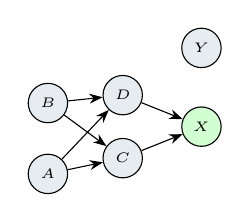
\begin{tikzpicture}[>=Stealth, font=\tiny,
	   v/.style={draw, circle, fill=blau-upc!12, inner sep=0pt, minimum size=5mm},
	   g/.style={draw, circle, fill=green!18, inner sep=0pt, minimum size=5mm}]
	  \node[v] (A) at (0,0) {$A$};
	  \node[v] (B) at (0,0.9) {$B$};
	  \node[v] (C) at (0.95,0.2) {$C$};
	  \node[v] (D) at (0.95,1.0) {$D$};
	  \node[g] (X) at (1.95,0.6) {$X$};
	  \node[v] (Y) at (1.95,1.6) {$Y$};
	  \draw[->] (A)--(C); \draw[->] (B)--(C); \draw[->] (A)--(D); \draw[->] (B)--(D); \draw[->] (C)--(X); \draw[->] (D)--(X);
	\end{tikzpicture}\\[1mm]
	{\tiny\itshape known pathways into $X$; $Y$ unlinked}\\[2.5mm]
	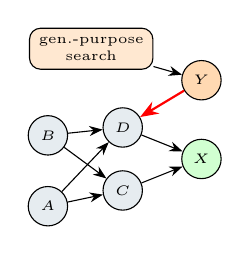
\begin{tikzpicture}[>=Stealth, font=\tiny,
	   v/.style={draw, circle, fill=blau-upc!12, inner sep=0pt, minimum size=5mm},
	   g/.style={draw, circle, fill=green!18, inner sep=0pt, minimum size=5mm}]
	  \node[v] (A) at (0,0) {$A$};
	  \node[v] (B) at (0,0.9) {$B$};
	  \node[v] (C) at (0.95,0.2) {$C$};
	  \node[v] (D) at (0.95,1.0) {$D$};
	  \node[g] (X) at (1.95,0.6) {$X$};
	  \node[v, fill=orange!30] (Y) at (1.95,1.6) {$Y$};
	  \draw[->] (A)--(C); \draw[->] (B)--(C); \draw[->] (A)--(D); \draw[->] (B)--(D); \draw[->] (C)--(X); \draw[->] (D)--(X);
	  \draw[->, red, thick] (Y)--(D);
	  \node[draw, rounded corners, fill=orange!18, font=\tiny, align=center] (gps) at (0.55,2.0) {gen.-purpose\\ search};
	  \draw[->] (gps)--(Y);
	\end{tikzpicture}\\[1mm]
	{\tiny\itshape learn $Y\!\to\!D\!\to\!X$; search targets $Y$}
	\end{center}
	\end{column}
	\end{columns}
}

\frame{\frametitle{Dualistic agents}
	\begin{block}{The cybernetic picture: Alexei plays a video game}
		{\tiny
		\begin{itemize}
			\item In the standard (``cybernetic'') picture, an agent learns by building a \textit{model} of its environment, and uses that model to plan towards a goal. This is Alexei, playing a video game:
    \begin{figure}
        \centering
        \includegraphics[width=0.27\linewidth]{fig/ekude8k13w2p8nm8mhfc.png}
        \label{fig:alexei}
    \end{figure}
        \item \textbf{Clear input \& output channels} between the agent and the environment
        \item The agent is \textbf{``larger'' than the environment}: it can hold a full copy of the game inside its own mind
        \item The agent is \textbf{``outside'' the environment}: it need not reason about itself, only about optimising the environment
        \item Standard idealised models of agency -- an expected-utility maximiser, or any agent that keeps a full internal model of the world and plans within it -- assume this dualistic, ``large agent'' picture
        \item But can we still reason about an agent that is \textit{smaller} than its environment, and contained inside it?
		\end{itemize}
		}
	\end{block}
}

\section{Embedded agents}
\frame{\frametitle{Embedded agents}
	\begin{block}{Embedded agents: Emmy plays real life}
		{\tiny
		\begin{itemize}
			\item This is Emmy. Emmy is playing real life:
    \begin{figure}
        \centering
        \includegraphics[width=0.27\linewidth]{fig/quqsoo5xeq4clo0wzjcf.png}
        \label{fig:emmy}
    \end{figure}
        \item The environment \textbf{contains her}: Emmy is just one part of the environment, made of the same pieces as everything else
        \item \textbf{No well-defined input/output channel} cleanly separating agent from environment
        \item She \textbf{cannot hold the environment inside her own head} -- the environment is bigger than she is
		\end{itemize}
		}
	\end{block}
}

\frame{\frametitle{Embedded agents}
	\begin{block}{Why embeddedness is hard}
		{\tiny
		\begin{itemize}
			\item The environment may contain \textbf{copies of her}, and other equally capable agents that model her while she models them
			\item She may be \textbf{modified, destroyed, or copied} (by herself or by others) between interaction steps
			\item Being inside the environment she manipulates, she is also capable of \textbf{self-improvement}
			\item Dualistic models struggle to represent this: a model that treats the environment as simpler than the agent itself cannot contain a copy of the agent, so it cannot describe an agent that is part of its own environment
			\item We would like a theory of consequentialist agency that is consistent with this embedded setting
		\end{itemize}
		}
	\end{block}
}


\frame{\frametitle{Self-Modification and Vingean Reflection}
	\begin{block}{Studying self-modification in a simplified setting}
		{\tiny
		\begin{itemize}
			\item We want to study \textbf{self-modification}: a sufficiently capable agent $A_1$ may rewrite its own code or build a successor $A_0$ more capable than itself (self-improvement is a special case of building a successor)
			\item Strategy: reduce this to a simpler setting we can analyse cleanly, but whose lessons should carry over to richer settings
			\item \textbf{Vingean uncertainty.} Here ``more capable'' means $A_0$ makes more accurate predictions, or selects more effective actions towards a goal, than $A_1$. So $A_1$ \textit{cannot} predict exactly what $A_0$ will do -- if it could, it could simply take those actions itself and be equally effective, and $A_0$ would not be more capable after all (cf.\ Deep Blue's designers knowing it was ``trying to win'' without knowing its moves)
			\item \textbf{Implication.} $A_1$ must establish, in an \textit{abstract} sense, that building $A_0$ is safe -- without simulating $A_0$ step by step
		\end{itemize}
		}
	\end{block}
	\begin{block}{The tiling principle}
		{\tiny
		\begin{itemize}
			\item We want $A_1$ to be able to approve building a successor \textit{similar to itself} -- e.g.\ the same algorithm running on different hardware
			\item This substrate-independence is the point: we want a \textit{robust} abstract argument (``constructing this successor is safe''), not a fragile rule that only blesses agents with identical source code
		\end{itemize}
		}
	\end{block}
}

\frame{\frametitle{Self-Modification: Why a Logical Framework?}
	\begin{block}{Stripping away empirical uncertainty}
		{\tiny
		\begin{itemize}
			\item A real-world agent also has \textbf{empirical uncertainty}: which environment am I in? how will my actions affect it?
			\item To isolate the self-trust problem, we \textit{strip this away}: assume the agent already knows its environment and how its actions influence it
			\item For simplicity, assume both the agent and the environment can be represented as \textbf{programs}
		\end{itemize}
		}
	\end{block}
	\begin{block}{Why proofs about programs are the right tool}
		{\tiny
		\begin{itemize}
			\item \textbf{Concrete behaviour becomes provable.} If a program halts and returns an output, $L$ can prove it -- the proof just lists the execution trace
			\item \textbf{But proofs also certify general behaviour.} One can prove a program never halts, or prove a universally quantified claim (``for all inputs, the output satisfies $X$'') -- things no single finite trace can show
			\item So once agents and environments are programs, proofs are \textit{strictly more general} than simulation: they let us certify a property \textit{in the abstract}, without inspecting the execution step by step -- exactly what Vingean uncertainty demands
		\end{itemize}
		}
	\end{block}
}

\frame{\frametitle{How can $A_1$ trust $A_0$?}
	\begin{block}{From ``$A_0$ acts on its proofs'' to ``$A_0$'s actions are safe''}
		{\tiny
		\begin{itemize}
			\item $A_1$ and $A_0$ share a satisficing goal $\mathcal{G}$, and $A_0$ only takes actions it can \textit{prove} achieve $\mathcal{G}$
			\item $A_1$ inspects $A_0$'s source code and verifies: if $A_0$ is constructed, then any action $A_0$ takes was proved (in $A_0$'s proof system) to achieve $\mathcal{G}$:
			$$A^1 \Vdash \bar{A}^0 \to (\forall b_i \in \textit{Acts}^0 : \bar{b}_i \to \Box_0[\bar{b}_i \to \mathcal{G}])  \qquad (2.3)$$
			{\scriptsize ($\bar{A}^0$ = ``$A_0$ is constructed'', \; $\Box_0[\phi]$ = ``a proof of $\phi$ exists in $A_0$'s system'')}
			\item But this only tells $A_1$ that $A_0$ \textit{acts on what its proof system certifies} -- not that what it certifies is actually \textit{true}
			\item To close this gap, $A_1$ needs to trust $A_0$'s proof system: whenever $A_0$ proves something, it is actually true
			$$A^1 \Vdash \forall b_i : (\Box_0[\bar{b}_i \to \mathcal{G}] \to (\bar{b}_i \to \mathcal{G})) \qquad (2.4)$$
			\item Combining (2.3) and (2.4): $\quad A^1 \Vdash \bar{A}^0 \to (\forall b_i \in \textit{Acts}^0 : (\bar{b}_i \to \mathcal{G}))$
			\\ {\scriptsize ``If $A_0$ is constructed, then any action $A_0$ takes achieves the goal''}
		\end{itemize}
		}
	\end{block}
}


\frame{\frametitle{The Löbian Obstacle}
	\begin{block}{The problem of self-trust}
		{\tiny
		\begin{itemize}
			\item When $A_1$ and $A_0$ use the \textit{same} proof system $L$, (2.4) becomes $\;L \vdash \forall \phi : (\Box \phi \to \phi)$: ``whatever I can prove is true'' -- $L$ vouching for its own proofs
			\item This conflates two distinct things. $L \vdash P$ means a concrete proof of $P$ is in hand. $\Box P$ is the \textit{internal} statement ``a proof of $P$ exists'', which $L$ can establish abstractly (e.g.\ by reasoning about a proof-search program) \textit{without exhibiting} any such proof
			\item \textbf{Löb's theorem.} For any statement $C$: if $L \vdash \Box C \to C$, then $L \vdash C$. The only statements $L$ can vouch for in the abstract are ones it can already prove outright
			\item E.g.\ self-trust would give $L \vdash \Box(2{+}2{=}5) \to (2{+}2{=}5)$, and Löb's theorem then forces $L \vdash 2{+}2{=}5$ -- impossible for a consistent $L$
			\item So a consistent system cannot trust its own proofs \textit{in the abstract}; it can only trust a proof once it has \textit{witnessed it directly}
		\end{itemize}
		}
	\end{block}

}

\frame{\frametitle{The Löbian Obstacle}
		\begin{block}{Consequence for tiling agents}
		{\tiny
		\begin{itemize}
			\item One workaround: $A_1$ can trust $A_0$'s proofs if $A_0$ uses a \textit{strictly weaker} proof system than $A_1$ (a stronger system can trust a weaker one)
			\item But then each successor in a chain must use a weaker system than its predecessor -- a ``telomere'' of logical strength that shortens with each generation
			\item Eventually the chain runs out of trust, so indefinitely long chains of safe self-modification seem blocked. The \textit{tiling agents} programme studies how, and whether, this obstacle can be overcome
		\end{itemize}
		}
	\end{block}

}

\frame{\frametitle{Embedded Subproblem: Logical Uncertainty}
	\begin{block}{Empirical vs.\ logical uncertainty}
		{\tiny
		\begin{itemize}
			\item \textbf{Empirical uncertainty:} ``will it rain tomorrow?'' -- we lack \textit{evidence} about the world; more observations would help
			\item \textbf{Logical uncertainty:} ``is the millionth digit of $\pi$ a 7?'' -- the answer is already fixed by the axioms of mathematics. We are not missing observations; we are missing \textit{computation}
			\item Other examples: the output of a program whose source code you already have, or whether a specific large number is prime
		\end{itemize}
		}
	\end{block}
	\begin{block}{Why this matters for embedded agents}
		{\tiny
		\begin{itemize}
			\item Standard Bayesian reasoning assumes \textit{logical omniscience}: the agent instantly knows all consequences of its beliefs, at no computational cost
			\item A bounded, embedded agent cannot: it may know every axiom of arithmetic yet still be uncertain about what they imply
			\item We need a principled way to assign probabilities to \textit{logical} facts, and to refine them as we spend more computation
		\end{itemize}
		}
	\end{block}
}

\frame{\frametitle{A Theory of Logical Uncertainty}
	\begin{block}{Analogy with Bayesian probability}
		{\tiny
		\begin{itemize}
			\item Bayesian probability gives us a \textit{model} of how an idealised agent should hold beliefs and make predictions under empirical uncertainty -- even though no real agent ever performs exact Bayesian inference
			\item We would like the same for \textit{logical} uncertainty: a clean account of how a bounded agent should assign and update probabilities over logical facts
		\end{itemize}
		}
	\end{block}
	\begin{block}{Modelling, then implementation}
		{\tiny
		\begin{itemize}
			\item Recall the modelling-vs-implementation split: a good \textit{theory} of logical uncertainty (the model) can then guide \textit{algorithms} that approximate it
			\item This mirrors how the theory of Bayesian inference guides practical, approximate inference algorithms (variational methods, MCMC, $\dots$)
		\end{itemize}
		}
	\end{block}
}

\frame{\frametitle{A Model of Logical (Computational) Uncertainty}
	\begin{block}{Ground truth vs.\ a time-bounded approximator}
		{\tiny
		\begin{itemize}
			\item \textbf{Ground truth:} a computable function $f$ from inputs to outputs (or output distributions)
			\item \textbf{Approximator:} a program $g$ that receives the input \textit{and} a string of random bits, and must answer within a fixed \textbf{time bound}. The random bits induce a distribution over $g$'s outputs; its quality is how close that distribution is to $f$
			\item \textbf{The tradeoff.} If computing $f$ needs a subroutine $h$ that $g$ cannot afford in time, a sensible move is to use the random bits to \textit{sample} a value $\hat h$ from a distribution over $h$'s output, and propagate that uncertainty forward
			\item As the time bound grows, $g$ can just compute $f$ directly and the random bits become irrelevant -- \textit{uncertainty shrinks as we spend computation}
		\end{itemize}
		}
	\end{block}
	\vspace{-1mm}
	\begin{center}
	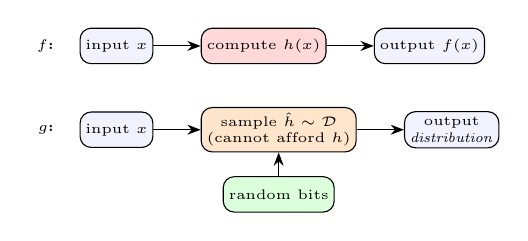
\begin{tikzpicture}[>=Stealth, font=\tiny,
	   box/.style={draw, rounded corners, align=center, inner sep=2pt, minimum height=4.5mm},
	   lbl/.style={font=\bfseries\tiny}]
	  \node[box, fill=blue!5] (gx) {input $x$};
	  \node[box, fill=red!15, right=6mm of gx] (gh) {compute $h(x)$};
	  \node[box, fill=blue!5, right=6mm of gh] (gf) {output $f(x)$};
	  \draw[->] (gx)--(gh); \draw[->] (gh)--(gf);
	  \node[lbl, left=2mm of gx] {$f$:};
	  \node[box, fill=blue!5, below=6mm of gx] (ax) {input $x$};
	  \node[box, fill=orange!20, right=6mm of ax] (ah) {sample $\hat h\sim\mathcal{D}$\\(cannot afford $h$)};
	  \node[box, fill=blue!5, right=6mm of ah] (af) {output\\ \emph{distribution}};
	  \draw[->] (ax)--(ah); \draw[->] (ah)--(af);
	  \node[box, fill=green!14, below=3mm of ah] (rb) {random bits};
	  \draw[->] (rb)--(ah);
	  \node[lbl, left=2mm of ax] {$g$:};
	\end{tikzpicture}
	\end{center}
}

\frame{\frametitle{Logical Uncertainty: Open Problems (I)}
	\begin{block}{An algorithm approximating itself}
		{\tiny
		\begin{itemize}
			\item Give one algorithm $A$ several possible time budgets. With a short budget, $A$ can try to approximate \textit{``what would I output if I had a larger budget?''}, using random bits in place of the computation it cannot afford
			\item So the same machinery models an agent reasoning about its own future, more-computed conclusions
		\end{itemize}
		}
	\end{block}
	\begin{block}{Randomness as logical counterfactuals}
		{\tiny
		\begin{itemize}
			\item In the subroutine picture, the random bits build a distribution over a subroutine's output: each draw is a different \textit{possibility} for what that output ``could'' be
			\item We need these possibilities precisely because we lack the compute to pin down the actual value -- so different settings of the random bits behave like different \textbf{logical counterfactuals}
		\end{itemize}
		}
	\end{block}
}


\frame{\frametitle{Logical Uncertainty: Open Problems (II)}
	\begin{block}{Which representations are useful?}
		{\tiny
		\begin{itemize}
			\item Suppose the approximator may also \textit{condition} on some side information about the input. Useful side information lets it reduce its logical uncertainty
			\item Handing it the output of an expensive subroutine saves that computation, freeing compute to reduce uncertainty elsewhere
			\item Handing it an \textit{encryption} of the input -- carrying the same Shannon / algorithmic information -- helps not at all
			\item So this gives a handle on which \textit{representations} of the same information are actually useful to a bounded reasoner, and on when ``post-processing'' a representation is worthwhile
		\end{itemize}
		}
	\end{block}
}
	
\frame{\frametitle{Aside: Logical Induction}
	\begin{block}{One concrete realisation of these ideas}
		{\tiny
		\begin{itemize}
			\item \textbf{Logical induction} (Garrabrant et al.) gives a computable way to assign probabilities to logical sentences that improve as more is proved. Picture a \textit{market} pricing each sentence $\varphi$ in $[0,1]$ (its probability); a $\varphi$-share pays \$1 once $\varphi$ is proved
			\item \textbf{The logical induction criterion:} no ``efficient'' (polynomial-time) trader can make unbounded profit against the market
			\item {\scriptsize (This weakens the classical Dutch-book argument -- ``\textit{no} trader can exploit you $\Rightarrow$ your beliefs obey the probability axioms'' -- to ``no \textit{efficient} trader can exploit you''; that single condition already implies many good properties.)}
			\item In the limit it yields: \textbf{coherence} (probability 1 to theorems, 0 to contradictions, monotone under implication); \textbf{statistical patterns} (it prices ``the $n$th digit of $\pi$ is 7'' near $10\%$ without computing it); and \textbf{self-trust} (current credence $=$ weighted average of its expected future credences)
		\end{itemize}
		}
	\end{block}
}


\section{Descriptive Agent Foundations}
\frame{\frametitle{Descriptive Agent Foundations}
	\begin{block}{From normative to descriptive}
		{\tiny
		\begin{itemize}
			\item \textbf{Normative (ideal) agent foundations:} characterizes how a perfectly rational agent \textit{should} reason and act in principle -- starts from desiderata of ideal agents and derives what follows
			\item \textbf{Descriptive agent foundations:} asks what agents we actually encounter in the wild actually \textit{look like} -- given any physical system (a neural network, a bacterium, a future AI), can we identify its goals, world-model, and decision-making structure?
			\item The aim is to develop concepts that apply to a wide range of intelligences, from bacteria to superintelligences
		\end{itemize}
		}
	\end{block}
	\begin{block}{World-centric framing and robustness to scale}
		{\tiny
		\begin{itemize}
			\item Normative agency starts from the agent's subjective viewpoint (beliefs, preferences, choice); embedded agency asks how that picture maps onto a world where the agent is just another physical subsystem
			\item Descriptive foundations starts from the other direction: from properties of the \textit{world} (modularity, selection pressures, resource constraints), it asks what processes reliably steer the world into narrow targets
			\item \textbf{Scaling up:} our concepts must not break when the agent becomes vastly more capable -- a safety property that fails under extreme optimisation pressure is useless
			\item \textbf{Scaling down:} the same framework should also degrade gracefully when applied to simpler systems
		\end{itemize}
		}
	\end{block}
}
\frame{\frametitle{Descriptive Agent Foundations}
	\begin{block}{Physical constraints shape agent structure}
		{\tiny
		\begin{itemize}
			\item Descriptive foundations emphasize selection pressures, constraints from the physical world, and computational boundedness -- these determine what kinds of agents actually arise
			\item  For instance, a key property of the world is \textbf{modularity}: the world decomposes into subsystems that interact sparsely. This should make both planning and world-modelling easier for any agent that exploits it
			\item \textbf{World-modelling:} Bayesian networks exploit modularity -- instead of maintaining a full joint hypothesis over every possible world, updates about variables are only propagated locally along edges in the graph
			\item \textbf{Planning:} General-purpose search exploits modularity -- if the world is modular, an agent can pursue decoupled subgoals independently, rather than having to plan everything jointly
		\end{itemize}
		}
	\end{block}
}


\frame{\frametitle{Optimization and Thermodynamics}
	\begin{block}{Optimization as local entropy reduction}
		{\tiny
		\begin{itemize}
			\item Powerful agents reliably steer the world towards narrow regions of target configurations -- outcomes that would be extremely unlikely to arise under any random process
			\item This is a form of \textit{local entropy reduction}: concentrating probability mass from a broad initial distribution onto a narrow final distribution around a target
			\item Irreversible transitions: funnelling many initial states into the same targets
			\item Existing results in stochastic thermodynamics such as fluctuation theorems (Second law of thermodynamics), cost of information erasure and information thermodynamics directly constrains the shape of optimization processes and hold far from equilibrium
		\end{itemize}
		}
	\end{block}
}

\frame{\frametitle{Optimization and Thermodynamics}
	\begin{block}{Even a pure predictor should attend to optimizers}
		{\tiny
		\begin{itemize}
			\item Even if you only want to predict the system's end state, it is useful to model the optimizers acting on it
			\item Without an optimizer: you must know the initial condition in detail and integrate the dynamics forward, and prediction error grows over time
			\item With an optimizer: the initial condition becomes irrelevant (it drives any starting state to its target), and the target itself is the prediction, robust to perturbations
			\item Paying attention to optimizers is efficient in terms of the information you have to learn vs what you get to predict
		\end{itemize}
		}
	\end{block}
}


\frame{\frametitle{Optimization  and Thermodynamics}
	\begin{block}{Steering costs information (Touchette \& Lloyd)}
		{\tiny
		\begin{center}
			\includegraphics[width=0.45\linewidth]{fig/lloyd.png}
		\end{center}
		\begin{itemize}
			\item A \textit{sighted} agent observes $X$ and chooses action $A$ accordingly; a \textit{blind} agent acts independently of $X$. The entropy reduction a sighted agent can achieve over the blind baseline is bounded:
			$$\Delta H \leq \Delta H_{\text{Blind}}^{\text{Max}} + I(X; A)$$
			\item The degree to which an agent can steer outcomes beyond what a blind policy achieves is paid for by the mutual information between its observations and its actions -- optimization requires information
		\end{itemize}
		}
	\end{block}
}

\frame{\frametitle{Optimization  and Thermodynamics}
	\begin{block}{From ensembles to individual states}
		{\tiny
		\begin{itemize}
			\item Traditional thermodynamics defines entropy in terms of probability distributions over ensembles -- but where does the distribution come from?
			\item \textbf{Algorithmic thermodynamics} (Ebtekar \& Hutter) replaces Shannon entropy $H$ with Kolmogorov complexity $K$, yielding thermodynamic laws that apply to \textit{individual physical states} rather than ensembles
            \item Intuitively, a state in which all particles are concentrated in one location would have low entropy, because the repeated coordinates can be printed by a short program.
		\end{itemize}
		}
	\end{block}
	\begin{block}{Knowledge as an endogenous physical resource}
		{\tiny
		\begin{itemize}
			\item In the Gibbs-Shannon framework, a distribution $\mu$ is an \textit{exogenous} parameter specifying what the agent knows. But an embedded agent's knowledge must be \textit{physically encoded} in its memory
			\item In algorithmic thermodynamics, knowledge becomes \textit{endogenous}: it manifests as \textbf{algorithmic mutual information} between the agent's memory and the environment
			\item This plays the same role as the mutual information in Touchette \& Lloyd: it is the resource an embedded agent can spend to steer the world into narrow target configurations
			\item So an agent that \textit{knows more} about its environment can perform \textit{more} optimization -- knowledge is the budget for steering
		\end{itemize}
		}
	\end{block}
}


\frame{\frametitle{Optimization  and Thermodynamics}
	\begin{block}{Why ``knowing more'' formally means ``optimizing more''}
		{\tiny
		\begin{itemize}
			\item Common intuition: an agent that understands its environment better can do more to it. Two bridges make this precise
			\item \textbf{Beliefs $\to$ mutual information.} If the agent's memory $a$ encodes a belief $q$ over environments, the true state $s$ has a Shannon codeword of length $\approx \log\frac{1}{q(s)}$, so its description given $a$ is short: $K(s \mid a) \leq \log\frac{1}{q(s)}$, hence
			$$I(a; s) = K(s) - K(s\mid a) \;\geq\; K(s) - \log\tfrac{1}{q(s)}$$
			\item \textbf{Mutual information $\to$ optimization.} By (the algorithmic) Touchette \& Lloyd, the agent can reduce the environment's entropy by up to $I(a; s)$
			\item \textbf{Together:} assigning more probability to the \textit{true} environment $\Rightarrow$ shorter description $\Rightarrow$ more mutual information $\Rightarrow$ more optimization. \emph{Knowing more is being able to do more} -- now a theorem, with a fixed exchange rate
		\end{itemize}
		}
	\end{block}
}


\end{document}